%%%%%%%%%%%%%%%%%%%%%%%%%%%%%%%%%%%%%%%%%%%%%%%%%%%%%%%%%%%%%%%%%%%%%%%%%%%%%%%%%%
\begin{frame}[fragile]\frametitle{}

\begin{center}
{\Large Named Entity Recognition (NER) with spaCy}

{\tiny (Ref: https://spacy.io/usage/spacy-101)}

\end{center}


\end{frame}


%%%%%%%%%%%%%%%%%%%%%%%%%%%%%%%%%%%%%%%%%%%%%%%%%%%%%%%%%%%%%%%%%%%%%%%%%%%%%%%%%%
\begin{frame}[fragile]\frametitle{spaCy}
  \begin{itemize}
  \item SpaCy is an open-source python library for NLP written in Python and Cython. 
	\item Offers pre-trained models for multi-language NER, as well as allowing developers to train and deploy custom NER models on domain specific corpuses. 
	\item SpaCy models are designed to be production-ready.
	\item Uses 1D residual convolutional neural networks (CNN) and incremental parsing with Bloom embeddings for NER
  \end{itemize}
	
\begin{center}
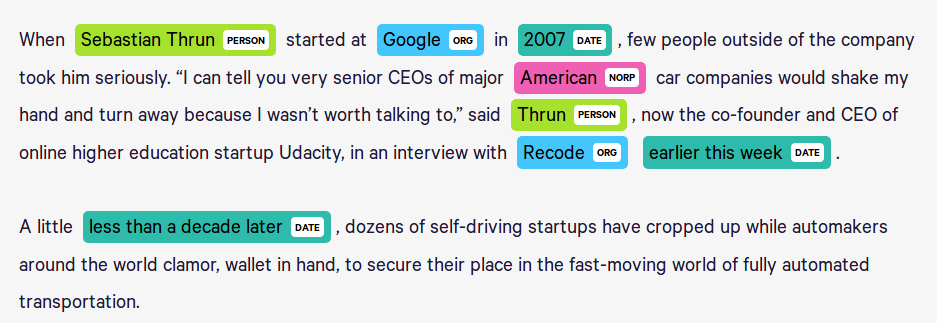
\includegraphics[width=0.8\linewidth,keepaspectratio]{spacy18}

	{\tiny (Ref: Complete Tutorial on Named Entity Recognition (NER) using Python and Keras - by Akshay Chavan)}

\end{center}
	
	{\tiny (Ref: Google Cloud AI Hub Named Entity Recognition using spaCy and Tensorflow)}
\end{frame}

%%%%%%%%%%%%%%%%%%%%%%%%%%%%%%%%%%%%%%%%%%%%%%%%%%%%%%%%%%%%%%%%%%%%%%%%%%%%%%%%%%
\begin{frame}[fragile]\frametitle{spaCy Default NER}
Identifies:
  \begin{itemize}
  \item PERSON:	People, including fictional
	\item ORG:	Companies, agencies, institutions, etc
	\item GPE:	Countries, cities, states
	\item PRODUCT:	Objects, vehicles, foods, etc. (Not services.)
	\item DATE:	Absolute or relative dates or periods
	\item TIME:	Times smaller than a day
	\item PERCENT:	Percentage, including ”%“
	\item MONEY:	Monetary values, including unit
	\item QUANTITY:	Measurements, as of weight or distance
	\item \ldots
  \end{itemize}
	
	{\tiny (Ref: Google Cloud AI Hub Named Entity Recognition using spaCy and Tensorflow)}
\end{frame}

%%%%%%%%%%%%%%%%%%%%%%%%%%%%%%%%%%%%%%%%%%%%%%%%%%%%%%%%%%%%%%%%%%%%%%%%%%%%%%%%%%
\begin{frame}[fragile]\frametitle{spaCy Default NER}

\begin{lstlisting}
import spacy
nlp = spacy.load('en_core_web_sm')

doc = nlp("Indians spent over $71 billion on clothes in 2018")
 
for ent in doc.ents:
    print(ent.text, ent.label_)
		
Indians NORP
over $71 billion MONEY
2018 DATE

spacy.explain("NORP")
Output: `Nationalities religious or political groups'
\end{lstlisting}
	
	{\tiny (Ref: spaCy Tutorial to Learn and Master Natural Language Processing (NLP) - Prateek Joshi - Analytics Vidhya)}
\end{frame}


%%%%%%%%%%%%%%%%%%%%%%%%%%%%%%%%%%%%%%%%%%%%%%%%%%%%%%%%%%%%%%%%%%%%%%%%%%%%%%%%%%
\begin{frame}[fragile]\frametitle{Named Entity Recognition NER}

\begin{lstlisting}
text = 'Apple is looking for buying a U.K. startup. Government has given permission.'

doc = nlp(text)
print(doc)

>> Apple is looking for buying a U.K. startup for $1 billion

for token in doc:
    print(token.text, token.label_)

Apple ORG
U.K. GPE
$1 billion MONEY

doc = nlp('Apple is looking for buying a UK startup for $1 billion in 2020')
displacy.render(doc, style = 'ent')
\end{lstlisting}

\begin{center}
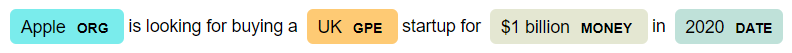
\includegraphics[width=0.8\linewidth,keepaspectratio]{spacy6}
\end{center}

\end{frame}

%%%%%%%%%%%%%%%%%%%%%%%%%%%%%%%%%%%%%%%%%%%%%%%%%%%%%%%%%%%%%%%%%%%%%%%%%%%%%%%%%%
\begin{frame}[fragile]\frametitle{Exercise}

  \begin{itemize}
    \item Process the text and create a doc object.
    \item Iterate over the doc.ents and print the entity text and label\_ attribute.
  \end{itemize}

  \begin{lstlisting}
import spacy

nlp = spacy.load("en_core_web_sm")

text = "It's official: Apple is the first U.S. public company to reach a $1 trillion market value"

# Process the text
doc = ____

# Iterate over the predicted entities
for ent in ____.____:
    # Print the entity text and its label
    print(ent.____, ____.____)
  \end{lstlisting}
	
\end{frame}

%%%%%%%%%%%%%%%%%%%%%%%%%%%%%%%%%%%%%%%%%%%%%%%%%%%%%%%%%%%%%%%%%%%%%%%%%%%%%%%%%%
\begin{frame}[fragile]\frametitle{}

\begin{center}
{\Large Custom NER}
\end{center}
\end{frame}

%%%%%%%%%%%%%%%%%%%%%%%%%%%%%%%%%%%%%%%%%%%%%%%%%%%%%%%%%%%%%%%%%%%%%%%%%%%%%%%%%%
\begin{frame}[fragile]\frametitle{Training your own NER}
  \begin{itemize}
  \item Either rule-based or machine learning (ML) based.
	\item Requires a large amount of labeled training data
	\item ML approaches from scratch: Hidden Markov Models, Maximum Entropy, and Conditional Random Fields, as well as deep learning approaches with Recurrent Neural Networks, such as Seq2Seq
	\item Need sentence inputs and annotated sentence outputs. 
	\item May also involve additional feature engineering
	\item Some libraries like spaCy and Stanford allow training of custom NER.
  \end{itemize}
\end{frame}


%%%%%%%%%%%%%%%%%%%%%%%%%%%%%%%%%%%%%%%%%%%%%%%%%%%%%%%%%%%%%%%%%%%%%%%%%%%%%%%%%%
\begin{frame}[fragile]\frametitle{NER Datasets}
  \begin{itemize}
  \item Domain-specific (i.e. Twitter, biomedical, advertising, news).
	\item i2b2 - Medication, treatments, diseases, risk factors, and medications
	\item CoNLL 2003 - English and german news articles annotated with location, organization, person, and miscellaneous
  \end{itemize}
\end{frame}


%%%%%%%%%%%%%%%%%%%%%%%%%%%%%%%%%%%%%%%%%%%%%%%%%%%%%%%%%%%%%%%%%%%%%%%%%%%%%%%%%%
\begin{frame}[fragile]\frametitle{NER Evaluation metrics}
  \begin{itemize}
  \item NER is most commonly evaluated with precision, recall, and F1-score.
  \end{itemize}
\end{frame}


%%%%%%%%%%%%%%%%%%%%%%%%%%%%%%%%%%%%%%%%%%%%%%%%%%%%%%%%%%%%%%%%%%%%%%%%%%%%%%%%%%
\begin{frame}[fragile]\frametitle{Training your own system}
  \begin{itemize}
  \item The feature extraction works almost identical as the one implemented in the Training a Part-Of-Speech Tagger, except need to add many features.
  \item Since the previous IOB tag is a very good indicator of what the current IOB tag is going to be, we have included the previous IOB tag as a feature.
  \item spaCy Provides Gold Parse method
  \item CRF++ can be used to generate custom NER tags.
  \end{itemize}
\end{frame}

%%%%%%%%%%%%%%%%%%%%%%%%%%%%%%%%%%%%%%%%%%%%%%%%%%%%%%%%%%%%%%%%%%%%%%%%%%%%%%%%%%
\begin{frame}[fragile]\frametitle{}

\begin{center}
{\Large spaCy Custom NER}
\end{center}
\end{frame}

%%%%%%%%%%%%%%%%%%%%%%%%%%%%%%%%%%%%%%%%%%%%%%%%%%%%%%%%%%
\begin{frame}[fragile]\frametitle{Custom NER Process}


\begin{center}
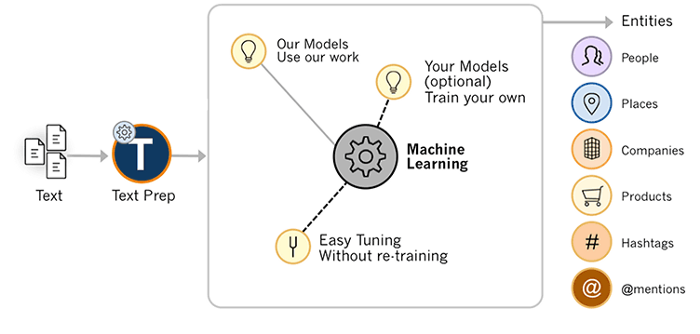
\includegraphics[width=0.8\linewidth,keepaspectratio]{ie15}
\end{center}

{\tiny (Ref: Training Custom NER - Nishanth N)}

\end{frame}

%%%%%%%%%%%%%%%%%%%%%%%%%%%%%%%%%%%%%%%%%%%%%%%%%%%%%%%%%%
\begin{frame}[fragile]\frametitle{Training Data Format}


\begin{lstlisting}

TRAIN_DATA = [
    ('Who is Nishanth?', {
        'entities': [(7, 15, 'PERSON')]
    }),
     ('Who is Kamal Khumar?', {
        'entities': [(7, 19, 'PERSON')]
    }),
    ('I like London and Berlin.', {
        'entities': [(7, 13, 'LOC'), (18, 24, 'LOC')]
    })
]
\end{lstlisting}

{\tiny (Ref: Training Custom NER - Nishanth N)}

\end{frame}

%%%%%%%%%%%%%%%%%%%%%%%%%%%%%%%%%%%%%%%%%%%%%%%%%%%%%%%%%%
\begin{frame}[fragile]\frametitle{NER Pipeline}


\begin{lstlisting}

nlp = spacy.load(model)  
ner = nlp.create_pipe('ner')
nlp.add_pipe(ner, last=True)

for _, annotations in TRAIN_DATA:
    for ent in annotations.get('entities'):
        ner.add_label(ent[2])
				
# Disable pipeline components you dont need to change
pipe_exceptions = ["ner", "trf_wordpiecer", "trf_tok2vec"]
unaffected_pipes = [pipe for pipe in nlp.pipe_names if pipe not in pipe_exceptions]

\end{lstlisting}

{\tiny (Ref: Training Custom NER - Nishanth N)}

\end{frame}

%%%%%%%%%%%%%%%%%%%%%%%%%%%%%%%%%%%%%%%%%%%%%%%%%%%%%%%%%%
\begin{frame}[fragile]\frametitle{Training}


\begin{lstlisting}
# Disable pipeline components you dont need to change
other_pipes = [pipe for pipe in nlp.pipe_names if pipe != 'ner']
with nlp.disable_pipes(*other_pipes):  # only train NER
    optimizer = nlp.begin_training()
    for itn in range(n_iter):
        random.shuffle(TRAIN_DATA)
        losses = {}
        for text, annotations in tqdm(TRAIN_DATA):
            nlp.update(
                [text],  
                [annotations],  
                drop=0.5,  
                sgd=optimizer,
                losses=losses)
        print(losses)
\end{lstlisting}

{\tiny (Ref: Training Custom NER - Nishanth N)}

\end{frame}

%%%%%%%%%%%%%%%%%%%%%%%%%%%%%%%%%%%%%%%%%%%%%%%%%%%%%%%%%%
\begin{frame}[fragile]\frametitle{Testing}


\begin{lstlisting}
doc = nlp("I was driving a Alto")
print("Entities", [(ent.text, ent.label_) for ent in doc.ents])
\end{lstlisting}

{\tiny (Ref: Training Custom NER - Nishanth N)}

\end{frame}